\section{Asking Adds a Late Signal That Grows With Scale}
\label{sec:question}

\begin{figure}[t]
  \centering
  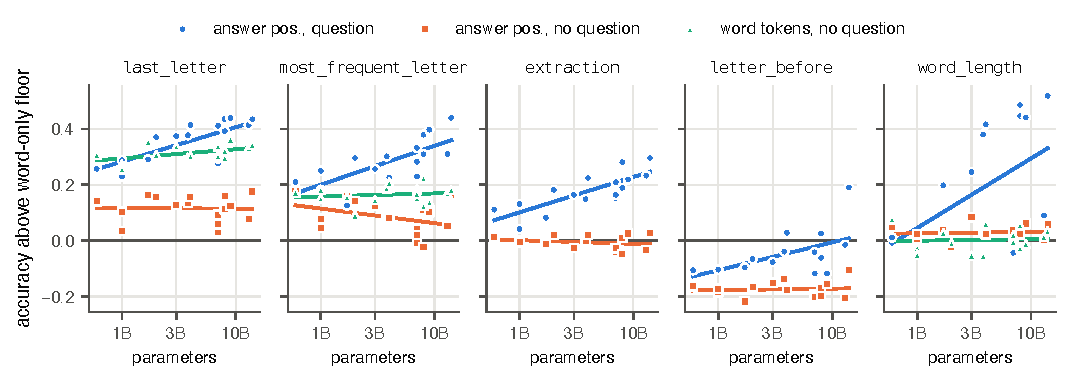
\includegraphics[width=\linewidth]{fig1_scaling_by_arm.pdf}
  \caption{Accuracy above the word-only floor against model size, zero shots, one point per model
    with an OLS line per arm. Answer position under the question (circles), answer position in the
    neutral sentence (squares), and, for the pure-word tasks, the word tokens in the neutral
    sentence (triangles; last-token read for \texttt{last\_letter} and \texttt{word\_length}, span
    mean for \texttt{most\_frequent\_letter}). Only the question arm rises with scale. The right
    panel contrasts a task with no word-level store: \texttt{word\_length} is assembled at the
    answer position (\S\ref{sec:store}). All values are in Table~\ref{tab:store} and the released
    analysis files.}
  \label{fig:scaling}
\end{figure}

\paragraph{The question effect grows with scale.}
Figure~\ref{fig:scaling} shows the four prompt-sensitive tasks, the tasks whose question-free
answer position retains little of the question arm's signal (below). Only the question arm rises
with scale; the neutral arm is flat or falling, and so is the word-level store. The interaction is
the slope of the per-model difference between the question and neutral arms
(Table~\ref{tab:interaction}). It is positive for all four tasks at both shot counts, survives Holm
correction across the four ($p_{\text{Holm}} \leq 0.015$), has a within-family slope of the same
size, and has a family-resampling interval that excludes zero.

\begin{table}[t]
  \centering\footnotesize
  \setlength{\tabcolsep}{3.2pt}
  \resizebox{\textwidth}{!}{\begin{tabular}{@{}lrrrrrrrrr@{}}
\toprule
 & & \multicolumn{4}{c}{all layers, held-out-selected} & \multicolumn{2}{c}{late ($\geq$0.5)} & \multicolumn{2}{c}{early ($\leq$0.25)} \\
\cmidrule(lr){3-6}\cmidrule(lr){7-8}\cmidrule(l){9-10}
task & shots & slope & $p$ (Holm) & within-fam. & family CI & slope & $p_{\text{Holm}}$ & slope & $p$ \\
\midrule
\texttt{last\_letter} & 0 & +0.126 & 0.0005 (0.002) & +0.125 & [+0.053, +0.159] & +0.162 & 0.0006 & $-$0.014 & 0.691 \\
\texttt{most\_frequent\_letter} & 0 & +0.192 & 0.0006 (0.002) & +0.173 & [+0.084, +0.241] & +0.202 & 0.0006 & $-$0.003 & 0.905 \\
\texttt{extraction} & 0 & +0.140 & 0.0001 (0.0004) & +0.160 & [+0.089, +0.183] & +0.138 & 0.0004 & $-$0.011 & 0.435 \\
\texttt{letter\_before} & 0 & +0.094 & 0.015 (0.015) & +0.104 & [+0.021, +0.170] & +0.091 & 0.015 & +0.004 & 0.710 \\
\addlinespace[2pt]
\texttt{last\_letter} & 3 & +0.132 & 0.0008 (0.003) & +0.129 & [+0.056, +0.186] & +0.151 & 0.004 & $-$0.005 & 0.924 \\
\texttt{most\_frequent\_letter} & 3 & +0.171 & 0.001 (0.003) & +0.157 & [+0.091, +0.266] & +0.205 & 0.0008 & $-$0.002 & 0.948 \\
\texttt{extraction} & 3 & +0.156 & 0.009 (0.009) & +0.192 & [+0.093, +0.271] & +0.151 & 0.014 & $-$0.007 & 0.672 \\
\texttt{letter\_before} & 3 & +0.135 & 0.002 (0.004) & +0.145 & [+0.079, +0.197] & +0.131 & 0.003 & $-$0.003 & 0.837 \\
\bottomrule
\end{tabular}}
  \caption{Question$\times$scale interaction: slope per decade of parameters of
    (question arm $-$ neutral arm) at the answer position. ``All layers'' uses held-out layer
    selection; the permutation $p$ is followed by its Holm-adjusted value across the four tasks.
    ``Late'' and ``early'' restrict each arm to layers at relative depth $\geq 0.5$ or $\leq 0.25$
    (maximum over the restricted layers); the late $p$ is Holm-adjusted across the four tasks.
    Family CI: 95\% interval from resampling model families.}
  \label{tab:interaction}
\end{table}

\paragraph{The growth is late.}
At zero shots the question arm's layer profile has two parts (Figure~\ref{fig:twophase}). In the
first quarter of the network it shows a bump at about 10\% depth that is similar in every model:
for \texttt{last\_letter} the early-band accuracy averages 0.75 and does not vary with scale
(slope $-0.002$ per decade, $p = 0.96$). One plausible source is the word's spelling being carried
to the adjacent answer token. Past half depth, larger models rise again and smaller models do not.
Restricting both arms to the late band leaves the interaction intact for every task
($p_{\text{Holm}} \leq 0.015$ at zero shots, $\leq 0.014$ at three); restricting them to the early
band removes it (all $|$slope$| \leq 0.014$, $p \geq 0.43$; Table~\ref{tab:interaction}). This also
answers a confound: the question prompt's answer token sits next to the word, while the neutral
sentence ends several tokens later. Distance could inflate the question arm early, but it is the
same in every model and cannot produce a scale trend, and the trend is absent where distance would
act.

\begin{figure}[t]
  \centering
  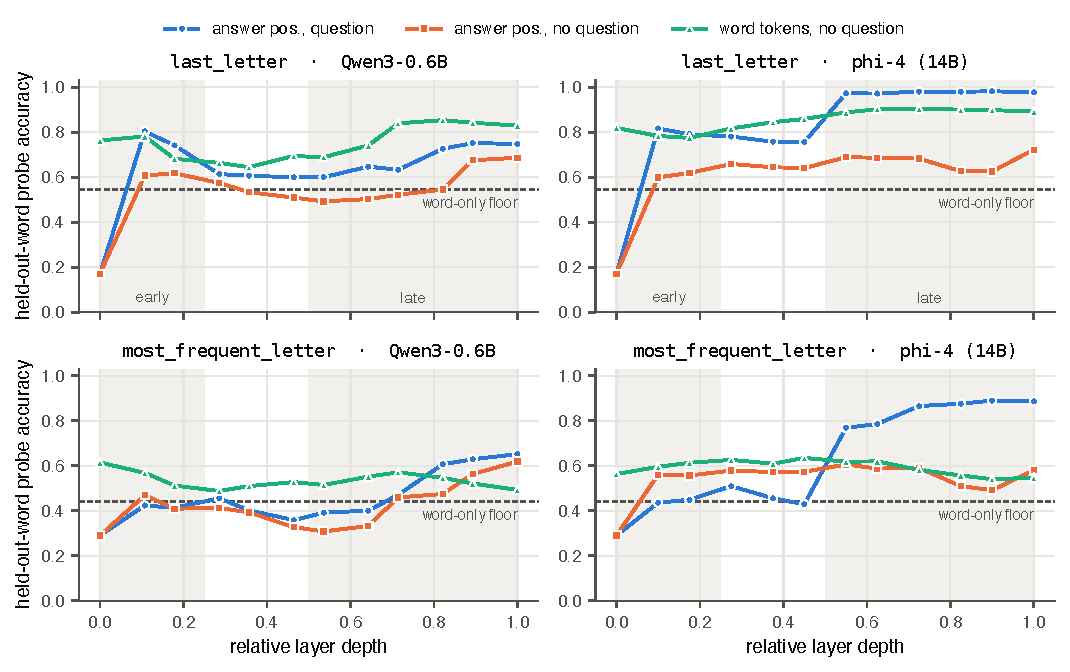
\includegraphics[width=\linewidth]{fig2_two_phase_profiles.pdf}
  \caption{Layer profiles at zero shots for the smallest model (Qwen3-0.6B) and the largest
    (phi-4). Shaded bands mark the early ($\leq 0.25$) and late ($\geq 0.5$) depth ranges used in
    Table~\ref{tab:interaction}; the dashed line is the word-only floor. The question arm's early
    bump is similar in both models; only the larger model's late phase rises well above the
    word-level store.}
  \label{fig:twophase}
\end{figure}

\paragraph{Large models exceed their store; small models fall short of it.}
The answer position under the question does not simply relay the word-level store. For
\texttt{last\_letter} at zero shots, Qwen3-0.6B's answer position is below its own store
($+0.257$ against $+0.307$ above the floor), while phi-4's is above it ($+0.434$ against
$+0.344$). The difference (answer position under the question minus store) grows with scale for
both store tasks: $+0.091$ per decade ($p = 0.017$) at zero shots and $+0.098$ ($p = 0.0007$) at
three for \texttt{last\_letter}; $+0.129$ ($p = 0.012$) and $+0.113$ ($p = 0.0016$) for
\texttt{most\_frequent\_letter}. The same holds within the late band. In the larger models the
answer position therefore carries more linearly decodable information about the property than
the word's own tokens do. Whether that excess reflects computation, integration across the word's
tokens, or a change of format that a linear probe can exploit, our measurements do not say.

\paragraph{Where the late rise begins.}
As an exploratory description, the first depth past the early band at which the question arm
exceeds the store becomes shallower with scale for \texttt{most\_frequent\_letter} at three shots
($r = -0.76$, $p = 0.0015$; median relative depth 0.77 in the smaller eight models, 0.59 in the
larger eight). The other three task--shot cells lean the same way without reaching significance
($p = 0.06$--$0.31$), and 12 probed layers limit resolution to about 0.08 of depth, so we do not
treat this as a finding.

\paragraph{What survives deleting the question.}
\emph{Retained} is the ratio of mean question-free accuracy to mean question accuracy, both measured
above a baseline (Table~\ref{tab:retained}). Against the majority class,
\texttt{last\_letter} retains half its signal at three shots (0.503). Against the word-only floor it
retains none ($-0.009$, continuation carrier 0.034); \texttt{extraction} retains none and
\texttt{most\_frequent\_letter} 5\%. The majority-baseline figure was length and letter-set information that
any word-level predictor has. At zero shots more survives (\texttt{last\_letter} 0.32), consistent
with the early bump, which reaches the sentence-final token of the neutral carrier only when no
demonstrations intervene. \texttt{first\_letter} and \texttt{contains\_letter} retain 64--92\% and
are not question-driven; \texttt{word\_length} retains 15--16\% and joins the question-driven group.

\begin{table}[t]
  \centering\footnotesize
  \setlength{\tabcolsep}{5pt}
  \begin{tabular}{@{}lrrrrrr@{}}
\toprule
 & \multicolumn{3}{c}{shots $=0$} & \multicolumn{3}{c}{shots $=3$} \\
\cmidrule(lr){2-4}\cmidrule(l){5-7}
task & majority & neutral & continuation & majority & neutral & continuation \\
\midrule
\texttt{extraction} & 0.228 & $-$0.036 & 0.240 & 0.151 & $-$0.000 & 0.017 \\
\texttt{last\_letter} & 0.671 & 0.324 & 0.473 & 0.503 & $-$0.009 & 0.034 \\
\texttt{most\_frequent\_letter} & 0.542 & 0.295 & 0.467 & 0.324 & 0.051 & 0.104 \\
\texttt{letter\_before} & 0.485 & -- & -- & 0.283 & -- & -- \\
\texttt{word\_length} & 0.546 & 0.149 & 0.439 & 0.416 & 0.162 & 0.175 \\
\texttt{counting\_lm} & 0.698 & 0.520 & 0.859 & 0.768 & 0.479 & 0.783 \\
\texttt{count\_distinct\_lm} & 0.911 & 0.911 & 1.082 & 0.673 & 0.673 & 0.610 \\
\texttt{first\_letter} & 0.885 & 0.811 & 0.855 & 0.856 & 0.758 & 0.696 \\
\texttt{contains\_letter} & 0.966 & 0.919 & 1.233 & 0.837 & 0.635 & 0.866 \\
\bottomrule
\end{tabular}
  \caption{Retained fraction of the question arm's signal when the question is deleted:
    mean(no-question $-$ base) / mean(question $-$ base). ``Majority'' uses the majority
    baseline and the neutral carrier; the other columns use the word-only floor. Missing values: the question arm's mean is not above the floor
    (\texttt{letter\_before}).}
  \label{tab:retained}
\end{table}
